%!TEX root = ../main.tex

\section{The KM mechanism and the CKM matrix}
\label{sec:cpviolation:kmmechanism}

Quarks get their mass through coupling to the Higgs field with vacuum
expectation value $v$ and via Yukawa interaction between the left-handed and
the right-handed quark content. The Yukawa matrices $\matr{Y}_d$ and
$\matr{Y}_u$ for down-type and up-type quarks involved in the corresponding
Lagrangian
\begin{align}
	\mathcal{L}_{\textrm{Yukawa}} = - \frac{v}{\sqrt{2}} (\bar{d}_{\mathrm{L}} \matr{Y}_d d_{\mathrm{R}} + \bar{u}_{\mathrm{L}} \matr{Y}_u u_{\mathrm{R}}) + \text{h.c.}
\end{align}
are not necessarily diagonal. The mass eigenstates $q^{\prime}$ can be
obtained by a unitary transformation
\begin{align}
	q^{\prime}_{\mathrm{A}} = \matr{V}_{\mathrm{A,}q}q_{\mathrm{A}} \quad \text{for } q = u,d \text{ and } \mathrm{A} = \mathrm{L,R}
\end{align}
with $\matr{V}_{\mathrm{A,}q}\matr{V}^\dagger_{\mathrm{A,}q} = 1$. When
applying this transformation in the Lagrangian that describes the
charged-current interaction
\begin{align}
	\mathcal{L}_{\textrm{CC}} &= -\frac{g_2}{\sqrt{2}}(\bar{u}_{\mathrm{L}}\gamma^{\mu}W_{\mu}^+ d_{\mathrm{L}} + \bar{d}_{\mathrm{L}}\gamma^{\mu}W_{\mu}^-u_{\mathrm{L}})\\
	&= -\frac{g_2}{\sqrt{2}}(\bar{u}^\prime_{\mathrm{L}}\gamma^{\mu}W_{\mu}^+\matr{V}_{\mathrm{L,}u}\matr{V}^\dagger_{\mathrm{L,}d}d^\prime_{\mathrm{L}} + \bar{d}^\prime_{\mathrm{L}}\gamma^{\mu}W_{\mu}^-\matr{V}_{\mathrm{L,}d}\matr{V}^\dagger_{\mathrm{L,}u}u^\prime_{\mathrm{L}})
\end{align}
the Cabibbo-Kobayashi-Maskawa matrix $\matr{V}_{\text{CKM}} =
\matr{V}_{\mathrm{L,}u}\matr{V}^\dagger_{\mathrm{L,}d}$ enters. As the
Yukawa matrices are not diagonalised by the same unitary transformation, the
CKM matrix is not the unit matrix and thus allows for flavour changes in the
weak interaction. So, the CKM matrix can be understood as the connection
between the mass eigenstates and the eigenstates to the weak interaction
\begin{align}
\begin{pmatrix}
d^\prime \\ s^\prime \\ b^\prime
\end{pmatrix}
=
\begin{pmatrix}
\Vud & \Vus & \Vub \\
\Vcd & \Vcs & \Vcb \\
\Vtd & \Vts & \Vtb \\
\end{pmatrix}
\begin{pmatrix}
d	\\	s	\\	b
\end{pmatrix}
\,.
\end{align}
Being the product of two unitary matrices the CKM matrix itself is unitary as
well. In general, a complex $3\times3$ matrix has 18 free parameters. However,
the unitarity removes nine of the degrees of freedom. Another five phases can
be constrained by global rephasings between the six mass fields. So, four free
parameters remain, of which three are real-valued angles and one is a complex
phase. This single phase introduces \CP violation to the SM. Kobayashi and
Maskawa developed this concept, which explains the origin of \CP violation and
predicted the existence of the third quark generation~\cite{Kobayashi:1973fv}.
The corresponding parametrisation of the CKM matrix is
\begin{align}
\matr{V}_{\text{CKM}} =
\begin{pmatrix}
c_1 & -s_1c_3 & -s_1s_3 \\
s_1c_2 & c_1c_2c_3 - s_2s_3e^{i\delta} & c_1c_2s_3 + s_2c_3e^{i\delta} \\
s_1s_2 & c_1s_2c_3 + c_2s_3e^{i\delta} & c_1s_2s_3 - c_2c_3e^{i\delta}
\end{pmatrix}
\,,
\end{align}
with $c_i$ and $s_i$ being shorthand for the cosine respectively sine of the
three Euler angles, and $\delta$ is the irreducible phase. Tests of the SM
concerning \CP violation in the quark mixing sector are performed by examining
the unitarity conditions of the CKM matrix. Six of the 12 equations are
orthogonality relations, which can be interpreted as triangles in the complex
plane. The area of all triangles is the same and given by half of the Jarlskog
invariant
\begin{align}
	J_{\CP} = \pm\,\mathcal{I}m (V_{ik}^{}V_{jl}^{}V_{il}^{\ast}V_{jk}^{\ast}) \quad (i \neq j, l \neq k)\,,
\end{align}
which expresses the amount of \CP violation in the
SM~\cite{Jarlskog:1985ht,*Jarlskog:1985cw}. It is measured to be $J = (3.04
^{+0.21}_{-0.20}) \times\num{e-5}$~\cite{PDG2016}. However, the ratios of the
side lengths of the unitarity triangles are very different. In two of them all
sides are of comparable length, one of the conditions is given by
\begin{align}
	\Vud\Vubs + \Vcd\Vcbs + \Vtd\Vtbs = 0\,.
\end{align}
When depicting the triangle in the complex plane it is convenient to scale the
triangle by dividing all side lengths by $\Vcd\Vcbs$. Then, the base matches
the real axis with length one as can be seen in
\cref{fig:cpviolation:ckmtriangle}.
\begin{figure}[htb]
\centering
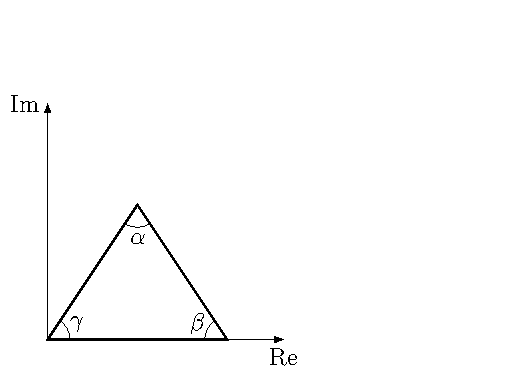
\includegraphics[width=0.5\textwidth]{03-CPViolation/tikz/pdf/CKMtriangle.pdf}
\caption{Schematic representation of the CKM unitarity triangle.}
\label{fig:cpviolation:ckmtriangle}
\end{figure}
Using the parametrisation of the CKM matrix by
Wolfenstein~\cite{Wolfenstein:1983yz}, which is an expansion in powers of
$\lambda \equiv |\Vus| = \num{0.2248\pm0.0006}$~\cite{PDG2016},
\begin{align}
\matr{V}_{\text{CKM}} =
\begin{pmatrix}
1 - \frac 12 \lambda^2 & \lambda & A\lambda^3(\rho - i\eta) \\
- \lambda & 1 - \frac 12 \lambda^2 & A\lambda^2 \\
A\lambda^3(1 - \rho - i\eta) & -A\lambda^2 & 1
\end{pmatrix}
+ \mathcal{O}(\lambda^4)\,,
\end{align}
the other two sides are given by
\begin{align}
	R_b &= \left(1 - \frac{\lambda^2}2\right)\frac 1\lambda \left|\frac \Vub\Vcb\right| = \sqrt{\bar{\rho}^2 + \bar{\eta}^2}\,,\label{eq:cpviolation:Rb}\\
	R_t &= \frac 1\lambda \left|\frac \Vtd\Vcb\right| = \sqrt{(1 - \bar{\rho})^2 + \bar{\eta}^2}\,,
\end{align}
where $\bar{\rho}$ and $\bar{\eta}$ define the position of the apex and are
related to the Wolfenstein parameters through
\begin{align}
	\bar{\rho} = \rho(1 - \lambda^2/2)\quad \text{and} \quad \bar{\eta} = \eta(1 - \lambda^2/2)\,.
\end{align}
The three angles of the unitarity triangle are defined by
\begin{align}
	\alpha \equiv \text{arg}\left(-\frac{\Vtd\Vtbs}{\Vud\Vubs}\right)\,,\quad
	\beta \equiv \text{arg}\left(-\frac{\Vcd\Vcbs}{\Vtd\Vtbs}\right)\,,\quad
	\gamma \equiv \text{arg}\left(-\frac{\Vud\Vubs}{\Vcd\Vcbs}\right)\,.
\label{eq:cpviolation:angles}
\end{align}

The unitarity triangle is overconstrained, \ie there are measurements of more
independent parameters than necessary to fully characterise the shape of the
triangle. The angle $\alpha$ can be studied with \BdToPiPi
decays~\cite{BaBar_alpha,Belle_alpha,LHCb-PAPER-2013-040}, $\beta$ is
precisely measured using the time-dependent \CP asymmetry in \BdToJPsiKS
decays (see \cref{sec:cpviolation:btoccbars}), and $\gamma$ can be extracted
from a combination of results in \BToDh decays~\cite{LHCb-CONF-2016-001}.
Semileptonic $b$-hadron decays are used to determine the size of the triangle
side $R_b$. Further information on $|\Vub|$ comes from studies of \BuToTauNu
decays~\cite{BaBar_BToTauNu,Belle_BToTauNu_HT,Belle_BToTauNu_SL}. The second
non-trivial side length $R_t$ is constrained by measurements of the mixing
frequencies \dmd and \dms in the system of neutral \Bd and \Bs
mesons~\cite{HFAG}. Furthermore, information on the position of the apex can
be gained from the measurement of \CP violation in the neutral kaon
system~\cite{PDG2016}. All these inputs are put into a global fit, which
mainly checks how well the different constraints agree on the position of the
apex. The latest result of the CKMfitter group in
\cref{fig:cpviolation:ckmtriangle_fitted} shows a very good agreement of all
present tests of \CP violation in the SM as the area for the position of the
apex is relatively small.
\begin{figure}
\centering
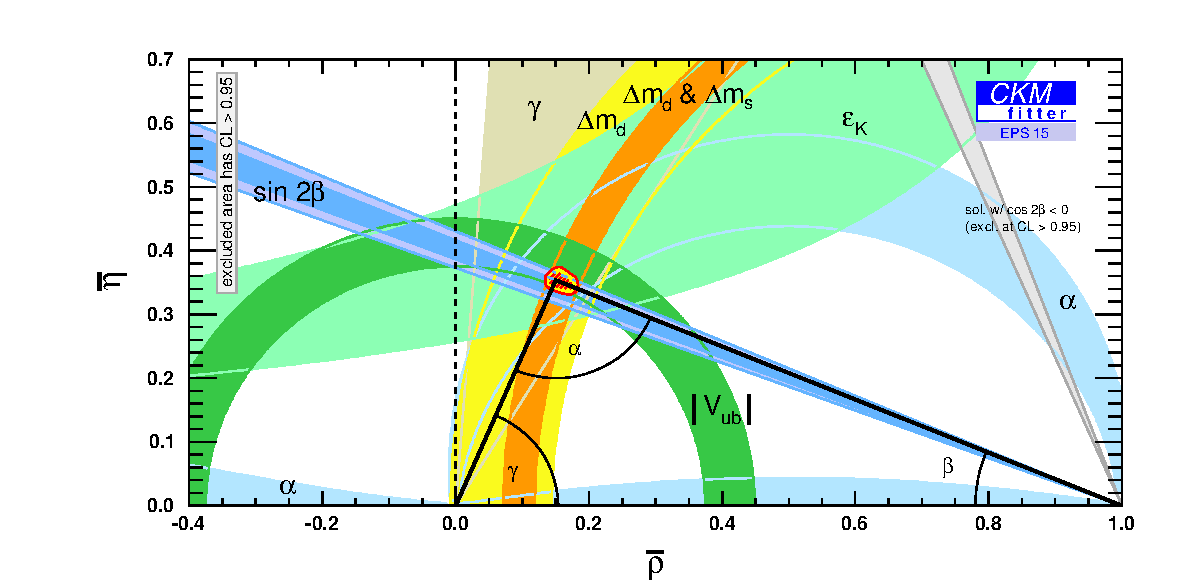
\includegraphics[width=\textwidth]{03-CPViolation/figs/CKMfitterTriangle.pdf}
\caption{Unitarity triangle with constraints from measurements of various
quantities~\cite{CKMfitter}.}
\label{fig:cpviolation:ckmtriangle_fitted}
\end{figure}
